

% Lecture Template for ME3023-001- Tristan Hill - Spring 2018 - Summer 2018
% 
% Measurements in Mechanical Systems

% Document settings
\documentclass[11pt]{article}
% \usepackage[margin=1in]{geometry}
\usepackage[left=1.5cm, right=1.5cm, top=2cm]{geometry}
\usepackage[pdftex]{graphicx}
\usepackage{multirow}
\usepackage{setspace}
\usepackage{hyperref}
\usepackage{color,soul}
\usepackage{fancyvrb}
\usepackage{framed}
\usepackage{wasysym}
\usepackage{multicol}

\usepackage[utf8]{inputenc}
\usepackage[english]{babel}
 


\pagestyle{plain}
\setlength\parindent{0pt}
\hypersetup{
    bookmarks=true,         % show bookmarks bar?
    unicode=false,          % non-Latin characters in Acrobat’s bookmarks
    pdftoolbar=true,        % show Acrobat’s toolbar?
    pdfmenubar=true,        % show Acrobat’s menu?
    pdffitwindow=false,     % window fit to page when opened
    pdfstartview={FitH},    % fits the width of the page to the window
    pdftitle={My title},    % title
    pdfauthor={Author},     % author
    pdfsubject={Subject},   % subject of the document
    pdfcreator={Creator},   % creator of the document
    pdfproducer={Producer}, % producer of the document
    pdfkeywords={keyword1} {key2} {key3}, % list of keywords
    pdfnewwindow=true,      % links in new window
    colorlinks=true,       % false: boxed links; true: colored links
    linkcolor=red,          % color of internal links (change box color with linkbordercolor)
    citecolor=green,        % color of links to bibliography
    filecolor=magenta,      % color of file links
    urlcolor=blue           % color of external links
}

% assignment number 
\newcommand{\NUM}{4} 
\newcommand{\VSpaceSize}{2mm} 
\newcommand{\HSpaceSize}{2mm} 

\definecolor{mygray}{rgb}{.6, .6, .6}
\definecolor{mypurple}{rgb}{0.6,0.1961,0.8}
\definecolor{mybrown}{rgb}{0.5451,0.2706,0.0745}
\definecolor{mygreen}{rgb}{0, .39, 0}

\newcommand{\R}{\color{red}}
\newcommand{\B}{\color{blue}}
\newcommand{\BR}{\color{mybrown}}
\newcommand{\K}{\color{black}}
\newcommand{\G}{\color{mygreen}}
\newcommand{\PR}{\color{mypurple}}

\newcommand{\Beta}{B}

\setulcolor{red} 
\setstcolor{green} 
\sethlcolor{mygray} 

\setlength{\parindent}{4em}
\setlength{\parskip}{1em}
\renewcommand{\baselinestretch}{1.5}


\begin{document}

\textbf{ \LARGE ME3023 Lecture -  Chapter \NUM \\\\ \hspace*{5mm} Probability and Statistics} \\\\
\textbf{ \hspace*{5mm}\underline{Theory and Design for Mechanical Measurements}\vspace{1mm}\\ 
                \hspace*{5mm} 5th ed. by Richard Figliola and Donald Beasley}\vspace{3mm}\\
\textbf{ \hspace*{5mm}Tristan Hill - Tennessee Technological University - Fall 2019} \vspace{3mm}\\

\begin{itemize}



		
	\item \textbf{ \LARGE 4.2 -  Statistical Measurement Theory  } \\\\
	\begin{itemize}

		\item \textbf{ \Large We want to estimate the {\bf \B true mean}, $x'$ from repeated measurement of $x$.} \\\\ 
		
		\item \textbf{ \Large The {\bf \B true mean}, $x'$ is the average of all possible values of $x$. We never actually get this!} \\\\ 
		
		\item \textbf{ \Large Through sampling we can find $\bar{x}$, the {\bf \G sample mean} value of $x$. We do get this!} \\\\ 
		
		\item \textbf{ \Large As our sample size increases, $\bar{x}$ approaches $x'$. } \\\\ 
		
		\scalebox{3}{$x'=\bar{x}\pm u_{\bar{x}}$}\\\\
		
		\item \textbf{ \Large Therefore, the sample mean $\bar{x}$ is the most probable estimate of the true mean $x'$. } \\\\ 
		
		\item \textbf{ \Large $\pm u_{\bar{x}}$ is the {\bf \PR uncertainty interval} in that estimate at some probability level, P\%. } \\\\ 
	
	         \item \textbf{ \Large The  {\bf \PR uncertainty interval} is the range about $\bar{x}$ that you would expect $x'$ to lie. } \\\\
		
\end{itemize}

		
		\newpage
		%\vspace{5mm}
		\item \textbf{ \LARGE 4.3 -  Statistical Measurement Theory  } \\
		
		\textbf{ \Large The true variance is:}\vspace{2mm}\\
		\scalebox{2}{$\sigma^2=\int\limits_{-\infty}^{\infty}(x-x')^2p(x)dx$} \\
		\begin{framed}
		\textbf{ \Large For discrete data the {\bf \B variance} is:}\\\\
		\scalebox{2}{$\sigma^2=\lim\limits_{N\rightarrow \infty}\frac{1}{N}\sum\limits_{i=1}^{N}(x_i-x')^2$}\\\\
		\textbf{\Large The {\bf \PR standard deviation} is the square root of the {\bf \B variance}.}\\\\
		\scalebox{2}{$\sigma=\sqrt{\sigma^2}$}\vspace{0mm}\\
		\end{framed}
		
		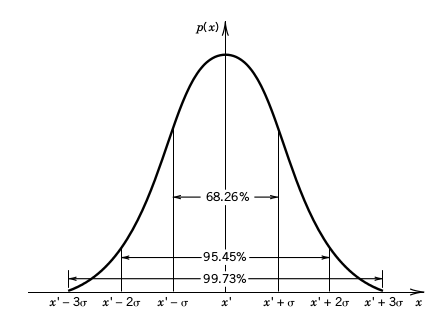
\includegraphics[scale=1.2]{lecture1_fig4.png}
		
		\newpage
		\item \textbf{ \LARGE 4.4 -  Statistics of Finite Sized Data Sets  } \\\\




\begin{itemize}

\item \textbf{ \Large We now try to predict the behavior of measured variable x based on a finite-sized sampling of x. We
do this by comparing the statistics from that sampling to an assumed probability density function for
the population. For example, if we recall the box of bearings discussed in Section 4.1, some two dozen bearings were measured, each having been randomly selected from a population numbering
in the thousands. So how do we use the resulting statistics from this sampling to characterize the
mean size and variance of all the bearings within the box? Within the constraints imposed by
probability and if we assume a probability density function for the population, it is possible to
estimate the true mean and true variance the population of all the bearings from the statistics of the
sampling. The method is now discussed. }\\

\item \textbf{ \Large  Suppose we examine the case where we obtain N measurements of x (that is, N repetitions),
each measurement represented by $x_i$ , where $i= 1, 2, . . . , N$ and $N$ is a finite value. In cases where
$N$ is not infinite or does not represent the total population, the statistical values calculated from such
finite data sets are only estimates of the true statistics of the population of $x$. We will call such
statistical estimates the finite statistics. An important point: whereas infinite statistics describe the
true behavior of the population of a variable, finite statistics describe only the behavior of the
sampled data set. }\\

\newpage
\item \textbf{ \Large Finite-sized data sets provide the statistical estimates known as: }

\begin{framed}
		\textbf{ \Large the {\bf \B sample mean:}}\\\\
		\scalebox{2}{$\bar{x}=\frac{1}{N}\sum\limits_{i=1}^{N}x_i$}\\\\
		\textbf{ \Large the {\bf \B Sample Variance:}}\\\\
		\scalebox{2}{$s_x^{2}=\frac{1}{N-1}\sum\limits_{i=1}^{N}(x_i-\bar{x})^2$}\\\\
		\textbf{\Large The {\bf \PR sample standard deviation} is the square root of the {\bf \B sample variance}.}\\\\
		\scalebox{2}{$s_x=\sqrt{s_x^2}$}\vspace{0mm}\\
		\end{framed}


\item \textbf{ \Large Did you notice that we divided by negative 1? } \\


\item \textbf{\Large The degrees of freedom, $\nu$, in a statistical estimate equate to the number
of data points minus the number of previously determined statistical parameters used in estimating
that value. For example, the degrees of freedom in the sample variance is $\nu=N-1$, as seen in
denominator of the equations above.} 

\newpage
\item \textbf{\Large The relation between probability and infinite statistics can be extended to data sets of finite
sample size with only some modification. When data sets are finite or smaller than the population,
the $z$ variable does not provide a reliable weight estimate of the true probability. However, the
sample variance can be weighted in a similar manner so as to compensate for the difference between
the finite statistical estimates and the statistics based on an assumed$p(x)$. For a normal distribution
of $x$ about some sample mean value, $x$, we can state that statistically} \\\\


\scalebox{2}{$x_i=\bar{x}\pm t_{\nu,P}s_x\hspace{5mm}(P\%)$}\vspace{0mm}\\ \\

\scalebox{2}{$t=\frac{\bar{x}-x'}{s_x/\sqrt{N}}$}

\newpage
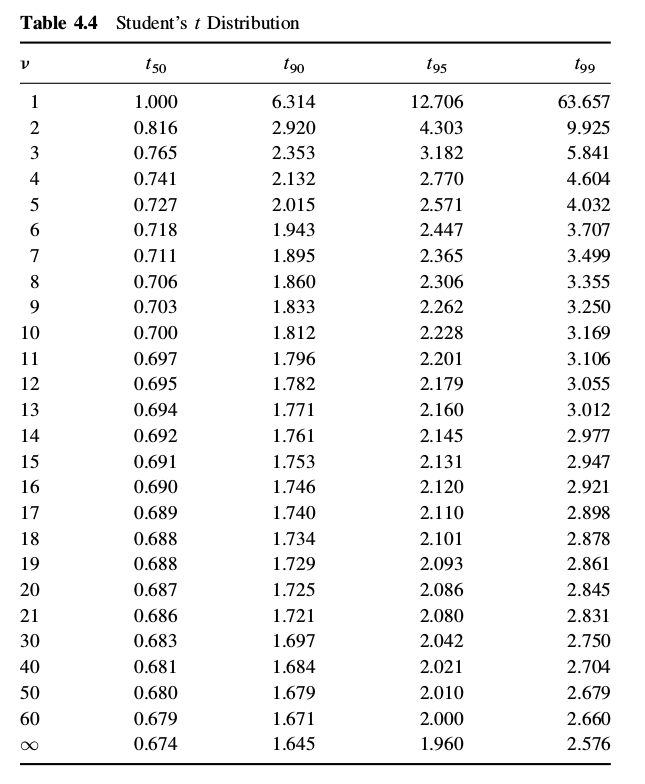
\includegraphics[scale=0.75]{lecture4_fig10.png} 


\newpage

\item \textbf{\Large Why do we divide by N-1 when calculating the sample statistical parameters? }
\end{itemize}

	\end{itemize}

\end{document}



